\subsection{Caso d'uso UC2: Apertura presentazione}
\begin{figure}[h] 
	\centering 
	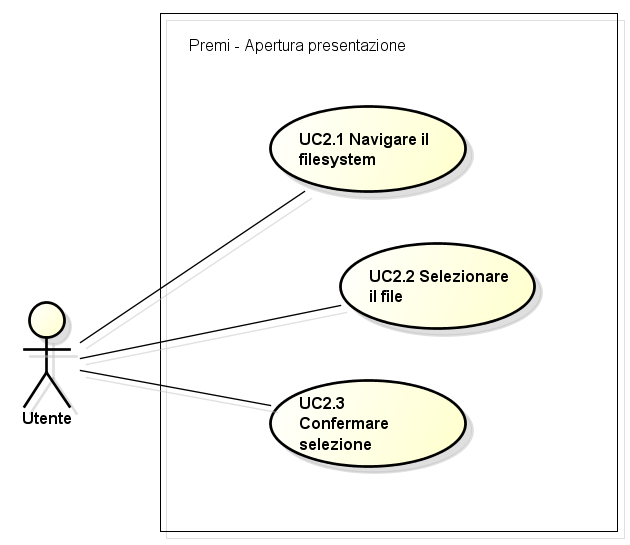
\includegraphics[scale=0.45] {img/UC2.png} 
	\caption{UC2 - Apertura presentazione} 
\end{figure}

\begin{itemize}
	\item \textbf{Attori:} Utente;
	\item \textbf{Scopo e descrizione:} L'utente ha scelto di aprire una presentazione già esistente. L'utente deve scegliere e selezionare la presentazione da aprire;
	\item \textbf{Precondizione:} Il sistema è in attesa che l'utente selezioni il file da aprire;
	\item \textbf{Flusso degli eventi:}
	\begin{enumerate}
		\item L'utente naviga il filesystem alla ricerca del file desiderato [UC2.1];
		\item L'utente seleziona il file [UC2.2];
		\item L'utente conferma la selezione [UC2.3].
	\end{enumerate}
	\item \textbf{Postcondizione:} Il sistema ha caricato il file selezionato dall'utente.
\end{itemize}

\subsection{Caso d'uso UC2.1: Navigare il filesystem}
\begin{itemize}
	\item \textbf{Attori:} Utente;
	\item \textbf{Scopo e descrizione:} L'utente può navigare il filesystem selezionando la cartella dentro la quale si trova il file da caricare;
	\item \textbf{Precondizione:} Il sistema è in attesa che l'utente selezioni una cartella;
	\item \textbf{Postcondizione:} Il sistema ha aggiornato la cartella corrente con quella selezionata dall'utente.
\end{itemize}

\subsection{Caso d'uso UC2.2: Selezionare il file}
\begin{itemize}
	\item \textbf{Attori:} Utente;
	\item \textbf{Scopo e descrizione:} L'utente deve selezionare il file che intende aprire;
	\item \textbf{Precondizione:} Il sistema mostra tutti i file contenuti nella cartella scelta in precedenza;
	\item \textbf{Postcondizione:} Il sistema evidenzia il file selezionato dall'utente.
\end{itemize}

\subsection{Caso d'uso UC2.3: Confermare selezione}
\begin{itemize}
	\item \textbf{Attori:} Utente;
	\item \textbf{Scopo e descrizione:} L'utente conferma la scelta del file fatta in precedenza;
	\item \textbf{Precondizione:} Il sistema ha selezionato il file scelto dall'utente;
	\item \textbf{Postcondizione:} Il sistema ha caricato il file scelto in precedenza dall'utente.
\end{itemize}